\chapter{System Description and Previous work}
\section{Description of System}
\subsubsection{Qubits}
A qubit is a quantum bit, the analog in quantum computing to the binary digit or bit of classical computing. Just as a bit is the basic unit of information in a classical computer, a qubit is the basic unit of information in a quantum computer. \citep{Whatisqubit} 
%\textbf{cite whatis}
\par
In simple words, a qubit is a two level quantum mechanical system.
%\newline \textbf{\emph{fig3}}
\begin{figure}[h]
\centering
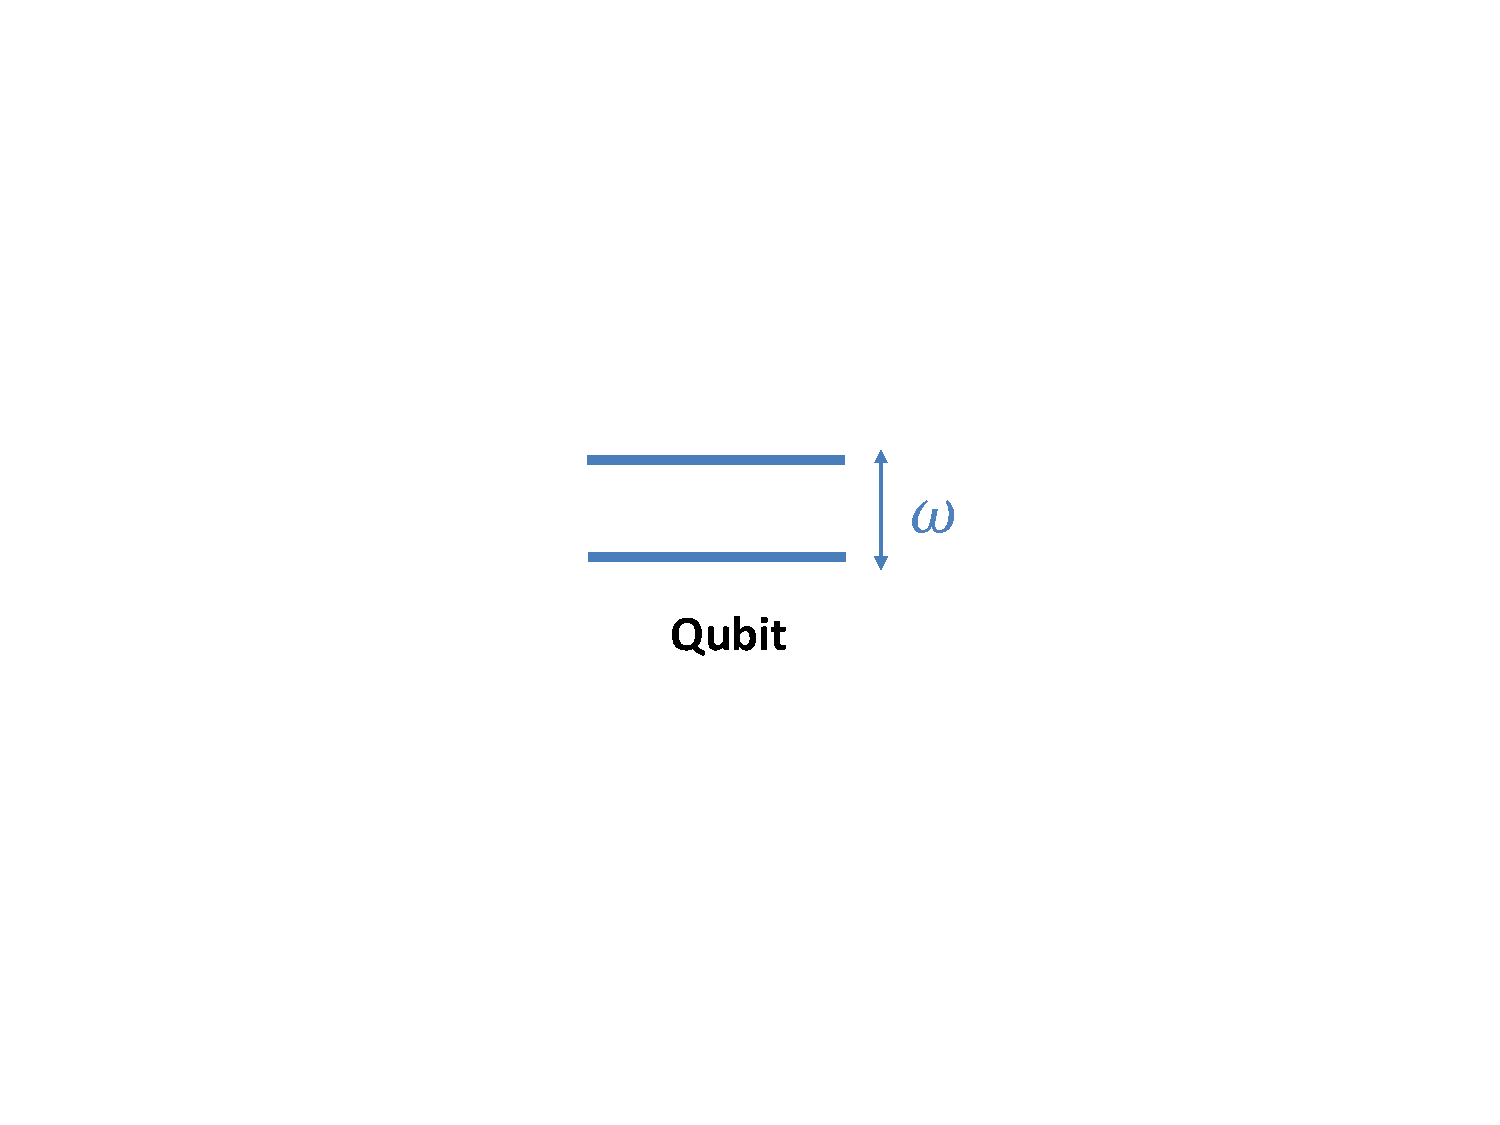
\includegraphics[width=0.5\textwidth]{Figr3a.pdf}
\caption{Qubit}
\label{fig:Figr3a}
\end{figure}


\subsubsection{Electromagnetic cavity}
An electromagnetic cavity  is an enclosure where standing electromagnetic waves can be sustained for considerable periods of time with or without an external driving field.%\citep{wiki:resonator}
%\textbf{ cite wiki resonator}
%\newline \emph{fig4}
\begin{figure}%[h]
\centering
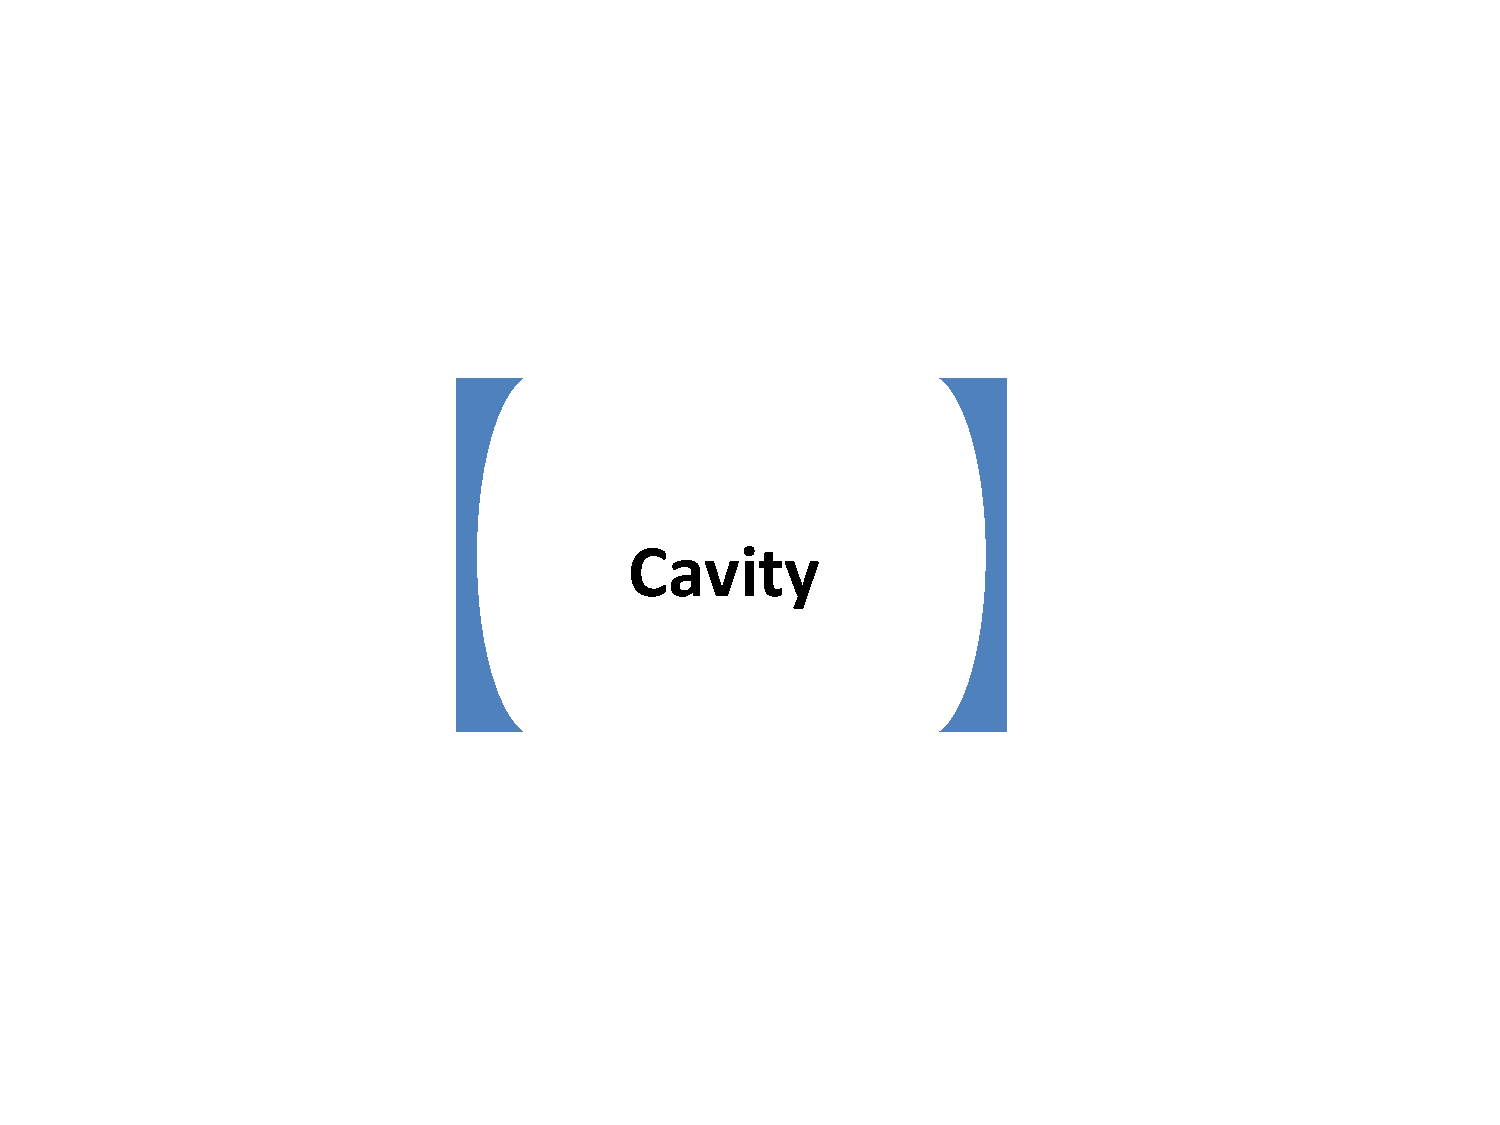
\includegraphics[width=0.5\textwidth]{Figr4a.pdf}
\caption{Cavity}
\label{fig:Figr4a}
\end{figure}

\subsubsection{Physics of system}
To exemplify how state transfer could be enhanced by tweaking the underlying Hamiltonian it would be better to do so by means of trying it out on an actual physical system. The physical system \citep{Tejas_APS1}  that we choose for this purpose is as follows : 
\begin{figure}[!h]
\centering
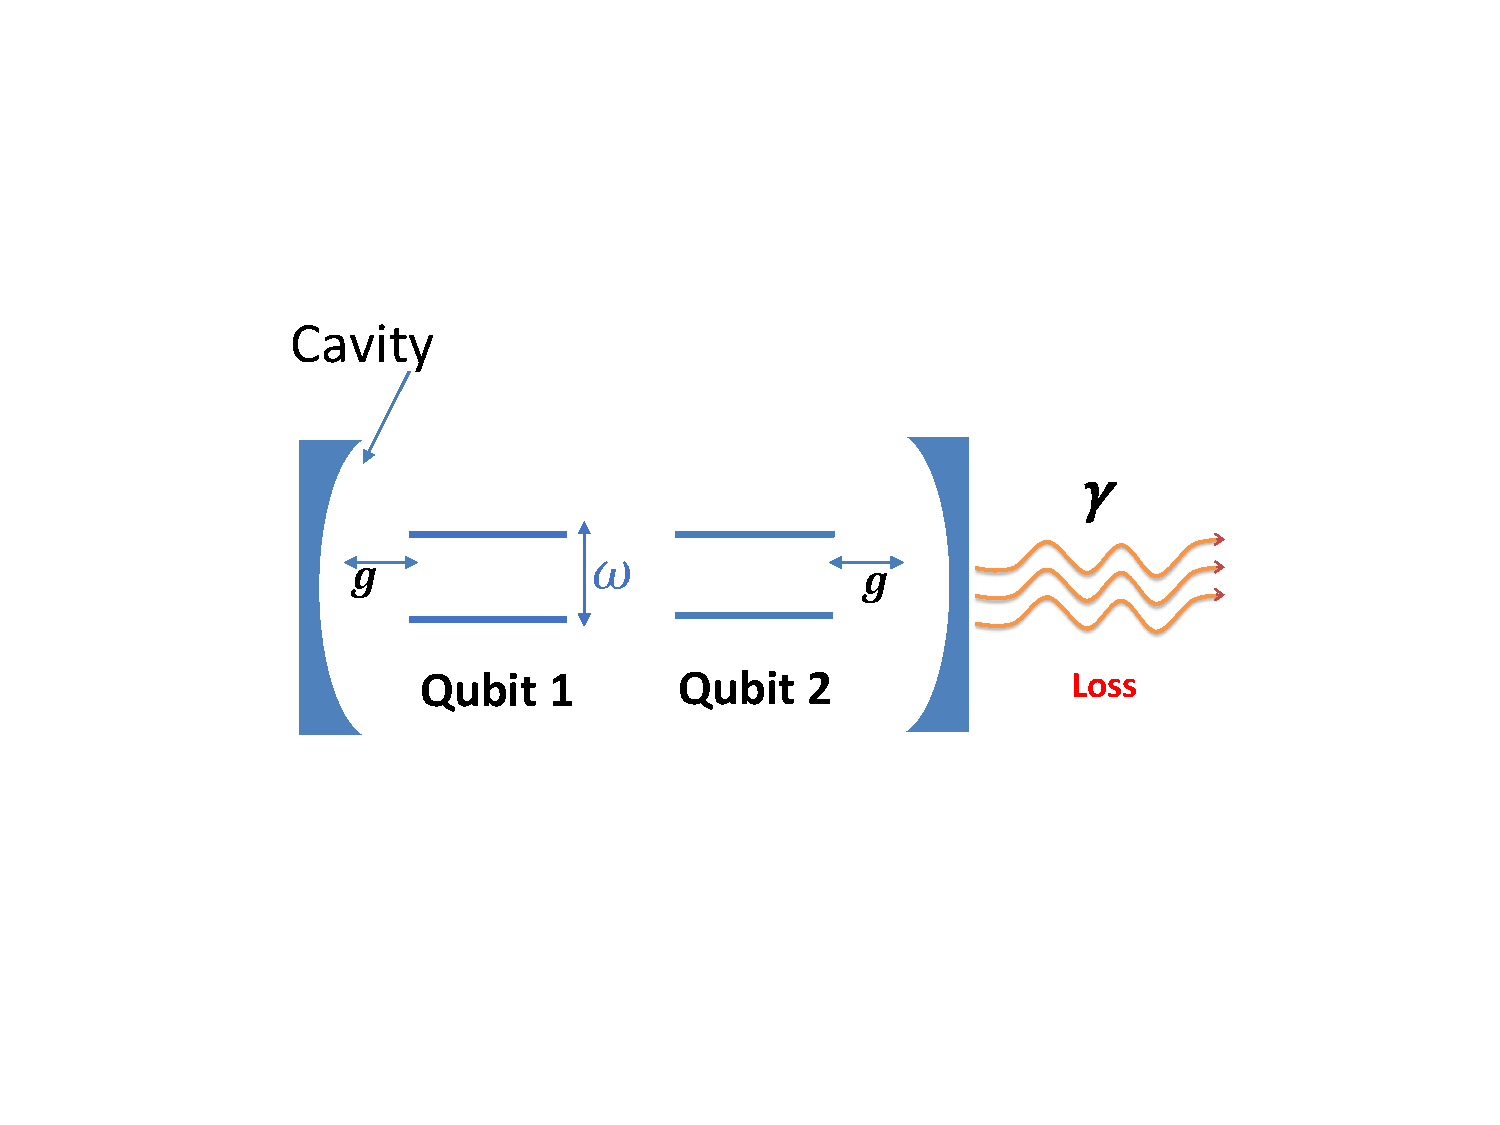
\includegraphics[width=0.8 \textwidth]{Figr1a.pdf}
\caption{Two qubits in a leaky cavity}
\label{fig:Figr1a}
\end{figure}


%The statement of the problem is as follows:
\begin{itemize}
\item We have:%\textbf{ cite my old aps }
\begin{enumerate}
\item Two qubits each with an energy difference of $(\hslash\thinspace{\omega})$.
\item A single mode lossy cavity approximated as a harmonic oscillator with energy spacing of $(\hslash\thinspace{\Omega})$.  
\end{enumerate}
\item Dissipation of quantum information occurs at a characteristic rate ($\gamma$).
\item There is no interaction between the qubits themselves.
\item Both the qubits are coupled to the cavity
\item The only way the qubits can communicate with each other is via the cavity
\end{itemize}

\section{Hamiltonian of the system}
The Hamiltonian of the system can be written as follows:
\begin{align}\label{eq:1}
H &= H_{0} + V
\end{align}
where $H_{0}$ is the bare Hamiltonian and $V$ is the coupling Hamiltonian. 
The bare Hamiltonian can be written as
\begin{align}\label{eq:2}
{H}_{0}&=\frac{\omega}{2}\thinspace{\sigma}_{z}\thinspace\otimes I^{(2)}\otimes{I^{(n)}}\thinspace + \thinspace\frac{\omega}{2}\thinspace{I^{(2)}}\thinspace\otimes\thinspace{\sigma}_{z}\otimes{I^{(n)}}\thinspace+\thinspace\Omega\thinspace I^{(2)}\otimes I^{(2)}\otimes{a}_{+}{a}_{- }
\end{align}
Where: 
\begin{itemize}
\item $\omega$ = frequency corresponding to the energy spacing  between the two levels of each qubit.
\item $\Omega$ = frequency corresponding to the difference in the energy levels of the cavity.
\item ${\sigma}_{z}, {\sigma}_{+}, {\sigma}_{-}$ =  Pauli matrices.   
\item ${a}_{+}, {a}_{-}$ = creation and annihilation operators for the cavity.
\item $I^{(2)}$ is the identity in the qubit Hilbert space.
\item $I^{(n)}$ is the identity in the harmonic oscillator Hilbert space.
\item $\hbar$ is set to be equal to $1$ in accordance with the usual practice. 
\end{itemize}
In the above equation~\eqref{eq:2} %\textbf{From2.2 }
\begin{itemize}
\item The first part represents bare Hamiltonian for the qubit 1.
\item The second part represents that of qubit 2.
\item The third  part represents that of  cavity. 
\end{itemize}

Now we will talk about how one would write down the interaction Hamiltonian $V$. Since, our system consists of qubits in a cavity effectively we have a double Jaynes Cummings type of Hamiltonian 
In our case since we have two qubits  we will have two couplings, \(g_{1}\) and \(g_{2}\). ${g}_{1}$ is the parameter related to the  strength of the coupling between the first qubit and the cavity. Similarly for ${g}_{2}$. So, following the discussion in the previous chapter we have 
\begin{align}\label{eq:15.1}
V &= V_{1} + V_{2}
\end{align}
Where: 
\begin{align}\label{eq 15.2}
V_{1}&= g_{1}\left({\sigma  }_{ - }\otimes I^{(2)}\otimes { a }_{ + }\thinspace + \thinspace{ \sigma }_{+}\otimes I^{(2)}\otimes{a}_{ - }\right)\\
V_{2}&= g_{ 2 }\left(I^{(2)}\otimes { \sigma  }_{ - }\otimes { a }_{ + }+I^{(2)}\otimes { \sigma  }_{ + }\otimes { a }_{ - }\right)
\end{align}


%\begin{itemize}
%\item $V_{1}= g_{1}\left({\sigma  }_{ - }\otimes I^{(2)}\otimes { a }_{ + }\thinspace + \thinspace{ \sigma }_{+}\otimes I^{(2)}\otimes{a}_{ - }\right)$
%\item $V_{2}= g_{ 2 }\left(I^{(2)}\otimes { \sigma  }_{ - }\otimes { a }_{ + }+I^{(2)}\otimes { \sigma  }_{ + }\otimes { a }_{ - }\right)$
%\end{itemize}

Putting all this together we get equation 
\begin{equation}\label{eq:16}
V= g_{1}\left({\sigma  }_{ - }\otimes I^{(2)}\otimes { a }_{ + }\thinspace + \thinspace{ \sigma }_{+}\otimes I^{(2)}\otimes{a}_{ - }\right)\thinspace
+\thinspace g_{ 2 }\left(I^{(2)}\otimes { \sigma  }_{ - }\otimes { a }_{ + }+I^{(2)}\otimes { \sigma  }_{ + }\otimes { a }_{ - }\right)
\end{equation}
Thus the full Hamiltonian is as follows:
\begin{multline}\label{FullH:1}
H =\frac{\omega}{2}\thinspace{\sigma}_{z}\thinspace\otimes I^{(2)}\otimes{I^{(n)}}\thinspace +\thinspace\frac{\omega}{2}\thinspace{I^{(2)}}\thinspace\otimes\thinspace{\sigma}_{z}\otimes{I^{(n)}}\thinspace+\thinspace\Omega\thinspace I^{(2)}\otimes I^{(2)}\otimes{a}_{+}{a}_{- } \\
+ g_{1}\left({\sigma  }_{ - }\otimes I^{(2)}\otimes { a }_{ + }\thinspace + \thinspace{ \sigma }_{+}\otimes I^{(2)}\otimes{a}_{ - }\right)\thinspace
+\thinspace g_{ 2 }\left(I^{(2)}\otimes { \sigma  }_{ - }\otimes { a }_{ + }+I^{(2)}\otimes { \sigma  }_{ + }\otimes { a }_{ - }\right)
\end{multline}
Where all the symbols are as defined earlier and $\hbar$ is set to be equal to $1$ in accordance with the usual practice.  
\subsubsection{Working of the system } 
This system works as follows:
\begin{itemize}
\item Qubit 1 is coupled to the cavity via the coupling Hamiltonian ${g}_{1}({\sigma  }_{ - }\otimes I^{(2)}\otimes { a }_{ + }\thinspace + \thinspace{ \sigma }_{+}\otimes I^{(2)}\otimes{a}_{ - })$. Through these coupling the state of qubit 1 is  being transferred to the cavity.
\item Similar to qubit 1, qubit 2 is also coupled via the coupling Hamiltonian ${g}_{2}\left(I^{(2)}\otimes { \sigma  }_{ - }\otimes { a }_{ + }+I^{(2)}\otimes { \sigma  }_{ + }\otimes { a }_{ - }\right)$. Through this coupling the information from the cavity is being transferred to qubit 2.
\item All this while the cavity is also leaking quantum information at a rate $\gamma$.
\end{itemize}

\subsection{Choice of Lindbladian operator}

Having derived the Lindblad equation in the previous chapter it is time to decide what would be the Lindbladian operators. One thing that we know is they must be of the same dimensions, shape etc. as that of the density matrix. This is because both of them live in the Hilbert space of the system.
\par 
We know that the cavity is a leaky one i.e. it undergoes spontaneous emissions. The cavity has been modelled as a harmonic oscillator. On undergoing emission the oscillator drops down from one fock state to the one below it. This is equivalent to the action of a annihilation operator acting on the harmonic space oscillator.
\par
Thus we can write 

\begin{align}\label{eq:1001}
L = I^{(2)} \otimes I^{(2)} \otimes {a}_{-}
\end{align}

where all the terms are the same as defined before 

\subsection{Putting it all together}
After all this hard work we end up with,

\begin{equation}\label{eq:1002}
\frac { {d\rho}_{s}}{dt} = -{ i\thinspace } [{ H },\thinspace { \rho  }_{ s }] +\gamma \left({ { L }\thinspace{ \rho}_{ s } }\thinspace { L }^{ \dagger  }-\frac { 1 }{ 2 } \{ { L }^{ \dagger}\thinspace{L},{\rho  }_{ s }\}\right)
\end{equation}

Where:
\begin{itemize}
\item $\rho_{s}$ = Density matrix for the system which includes both the qubits and the cavity.
\item  Total Hamiltonian as written in \eqref{FullH:1}\begin{multline}\notag
H =\frac{\omega}{2}\thinspace{\sigma}_{z}\thinspace\otimes I^{(2)}\otimes{I^{(n)}}\thinspace +\thinspace\frac{\omega}{2}\thinspace{I^{(2)}}\thinspace\otimes\thinspace{\sigma}_{z}\otimes{I^{(n)}}\thinspace+\thinspace\Omega\thinspace I^{(2)}\otimes I^{(2)}\otimes{a}_{+}{a}_{- } \\
+ g \left({\sigma  }_{ - }\otimes I^{(2)}\otimes { a }_{ + } + { \sigma }_{+}\otimes I^{(2)}\otimes{a}_{ - }
+ I^{(2)}\otimes { \sigma  }_{ - }\otimes { a }_{ + }+I^{(2)}\otimes { \sigma  }_{ + }\otimes { a }_{ - }\right)
\end{multline} where we have additionally set $g_{1}$ equal to $g_{2}$ and replaced both of them by $g$, since this is the case which we could consider while performing the numerical calculations. Here $g$ is the common coupling strength of the qubits to the cavity.
\item $ {L} = I^{(2)} \otimes I^{(2)} \otimes {a}_{-} $  Lindbladian operator as in \eqref{eq:1001}
\item $\gamma$ = Characteristic rate of dissipation for the cavity. 
\item $\hbar$ is set to be equal to $1$ in accordance with the usual practice. 
\end{itemize}




